\chapter{User Trial Evidence}
\label{appendix:user-trials}

The prepared mission conditions and numerical allocations are purely illustrative, as their only purpose is to provide common starting points for the timed tasks.
The inputs are utilized as values for the corresponding properties of the MBSE models.

{\small
\setlength{\tabcolsep}{4pt}
\setlength{\parskip}{0pt}
\renewcommand{\arraystretch}{1.06}
\begin{longtable}{@{}>{\raggedright\arraybackslash}p{0.20\linewidth}>{\raggedright\arraybackslash}p{\dimexpr0.80\linewidth-2\tabcolsep\relax}@{}}
\caption{Illustrative inputs shared by the prepared sizing tasks. Changes for each task are given in Table~\ref{tab:user-trial-task-sheets}. Groups are illustrative.}\label{tab:user-trial-initial-inputs}\\
\toprule
\textbf{Group} & \textbf{Prepared values} \\
\midrule
\endfirsthead
\toprule
\textbf{Group} & \textbf{Prepared values} \\
\midrule
\endhead
\bottomrule
\endfoot
Mission and orbit & 1U bus, lifetime 2~years, 365.25~days/year, altitude 600~km, eccentricity 0.05, beta angle $0^\circ$, Sun projection angle $30^\circ$, Earth radius 6378~km and gravitational parameter 398601~km$^3$/s$^2$. \\
Attitude & Ideal Sun pointing with the $+Z$ face toward the Sun and the array mounted on $+Z$. \\
EPS loads and accounting & Sunlight and eclipse mean loads 5 and 3~W. Delivered energy allocations 25000 and 8000~J. Each of the four default EPS components has mass 0.1~kg and volume 0.0001~m$^3$. \\
Array electrical inputs & 6S4P, EOL cell voltage 2.3~V, EOL cell current 0.45~A, open-circuit cell voltage 2.6~V and short-circuit cell current 0.5~A. Sunlight and eclipse path efficiencies 0.8 and 0.65. Ideal MPPT through the regulator and converter. \\
Array area and illumination & Cell active area 0.00345~m$^2$, packing fraction 0.9, usable area 0.1~m$^2$, BOL efficiency 0.32, lifetime retention 0.9375, temperature factor 1, irradiance 1000~W/m$^2$, inherent retention 1 and assembly efficiency 1. \\
Battery & 1S2P. Cell ratings 3.7~V, 2.75~Ah and 10.175~Wh. Cell voltage interval 3.0--4.2~V. Cell charge and discharge limits 1 and 3~A. Cycle law coefficient 2000, exponent $-1$ and characterized DoD interval 0.1--0.8. Degradation margin 0.2. Energy and capacity retention 0.8. \\
Receiving limits & Converter input interval 6--18~V, absolute maximum input 22~V and maximum input current 2.5~A. Output 5~V and maximum output current 3~A. Battery receiving interval 2.8--4.3~V. Required battery charge and discharge currents 1 and 2~A. \\
Load rail & Instrument mass 0.01~kg and volume 0.00001~m$^3$. Active on state 5~V and 1~A, off state 0~V and 0~A. The bus voltage and current checks link this on state to the converter output ratings. \\
\end{longtable}}

\section{Task presentations}

{\small
\setlength{\tabcolsep}{4pt}
\setlength{\parskip}{0pt}
\renewcommand{\arraystretch}{1.06}
\begin{longtable}{@{}>{\raggedright\arraybackslash}p{0.10\linewidth}>{\raggedright\arraybackslash}p{\dimexpr0.90\linewidth-2\tabcolsep\relax}@{}}
\caption{Task inputs and requested submissions. Each role receives a separate copy of the same initial mission for each task.}\label{tab:user-trial-task-sheets}\\
\toprule
\textbf{MOP} & \textbf{Prepared state and task} \\
\midrule
\endfirsthead
\toprule
\textbf{MOP} & \textbf{Prepared state and task} \\
\midrule
\endhead
\bottomrule
\endfoot
01 & Given MR\_BASE, which limits EPS mass to 0.6~kg, create MR\_CHILD at mission level. Its parent is MR\_BASE and its child list is empty. Limit battery mass to 0.12~kg through a condition named maximum, with measure linked to battery mass and predicate measure $\leq$ target. Retain the rationale ``Reserve 0.48~kg for the other EPS components,'' verification method Analysis, resolution status Resolved and unresolved field reason None. The identifier is the requirement name. Parent and child identifiers, method and resolution information use explicit requirement parameters. Save and reopen the requirement, then submit its fields and condition result. \\
02 & Retrieve MR\_PARENT's forward links to MR\_ARRAY and MR\_BATTERY, their allocations to SolarArray and Battery, and each child's reverse link to MR\_PARENT. The prepared links use parent, child and component identifier parameters. Submit the associated identifiers without changing them. \\
03 & Inspect analysis\_complete, with 2~W multiplied by 5~s, and analysis\_failed, which deliberately divides 2~W by zero seconds. Both retain a link to MR\_ENERGY, a method description, a synthetic nominal scenario and their input bindings. Submit the available result views and execution states. Report any limitation in retrieving retained execution records. \\
04 & Reload the retained sizing mission through Reopen and rerun sunlight\_energy and solar\_power through their stored bindings. Submit the rerun results. The prepared environment supplies the framework dependency. \\
05 & Fill seven prepared allocation parameters. Assign generation to SolarArray, storage to Battery, conversion and regulation to RegulatorAndConverter, and protection, distribution and control to PowerCircuit. Save each assignment and submit the mission requirement table. The retained component identifier appears in each requirement statement. \\
06 & Apply four separate baseline variations. Change lifetime from 2 to 1~year, eclipse mean load from 3 to 4~W, battery parallel count from 2 to 3, and Earth radius from 6378 to 6371~km. Restore each preceding edit before the next variation. Capture intermediate EPS result views for each variation and submit the final variation's result view. \\
07 & The array's EOL cell current is omitted. Identify the missing quantity through the generated solar\_cell\_count requirement, supply 0.45~A, save and submit the updated requirement. \\
08 & Inspect the generated solar\_cell\_count requirement. Submit its required count calculation, required power and cell power mappings, and minimum verification condition. Preserve the expressions and inputs. \\
09 & Use the GUI and terminal in the prepared mission repository to save an authored baseline with the decision rationale ``Approved by trial coordinator for this synthetic demonstration, retain the 600~km baseline.'' Use author Trial Operator. Change altitude from 600 to 650~km in the GUI, inspect Git status and the diff using the briefed commands, retrieve the baseline through Git and reopen it. Submit the retained requirement, mission, design and model revision identifiers R0, M0, D0 and A0 and the decision history. These are illustrative revision labels. \\
11 & Query the battery alternatives in Table~\ref{tab:user-trial-battery-alternatives}. The generic battery's direct requirements demand minimum rated energy 11~Wh, maximum mass 0.075~kg and nominal voltage 3.6~V. Find all matches and sort by rated energy, highest first. Submit the part numbers and leave the live battery unassigned. \\
13 & Start from a blank mission input sheet with the bus, instrument, modes and allocation rows already created. Enter lifetime 2~years, 365.25~days/year, altitude 600~km, eccentricity 0, beta angle $0^\circ$, Sun pointing on $+Z$, and irradiance 1000~W/m$^2$. Set nominal orbital fraction and the instrument's nominal mode share to 1, and on/off state shares to 0.2/0.8. Set the on state to 5~V and 1~A and the off state to 0~V and 0~A. Reopen and submit retained inputs. A prepared requirement statement displays their bindings without inferring chronology or averaging. \\
\end{longtable}}

\begin{table}[htbp]
\centering
\small
\caption{Catalogue values supplied to MOP-11. The supplied energy values are minimum ratings and the masses are maximum ratings. Every candidate has nominal voltage 3.6~V.}
\label{tab:user-trial-battery-alternatives}
\begin{tabular}{@{}lrr@{}}
\toprule
\textbf{Molicel part number} & \textbf{Energy (Wh)} & \textbf{Mass (kg)} \\
\midrule
\href{https://www.molicel.com/wp-content/uploads/INR18650M30A-V2-80088.pdf}{INR-18650-M30A} & 10.4 & 0.048 \\
\href{https://www.molicel.com/wp-content/uploads/INR18650M35A_1.4_Product-Data-Sheet-of-INR-18650-M35A-80096.pdf}{INR-18650-M35A} & 11.9 & 0.048 \\
\href{https://www.molicel.com/wp-content/uploads/INR21700P42A_1.7_Product-Data-Sheet-of-INR-21700-P42A-80092.pdf}{INR-21700-P42A} & 14.7 & 0.070 \\
\href{https://www.molicel.com/wp-content/uploads/INR21700P45B_1.4_Product-Data-Sheet-of-INR-21700-P45B-80109.pdf}{INR-21700-P45B} & 15.5 & 0.070 \\
\href{https://www.molicel.com/wp-content/uploads/INR18650P26A_1.4_Product-Data-Sheet-of-INR-18650-P26A-80087.pdf}{INR-18650-P26A} & Unknown & 0.050 \\
\bottomrule
\end{tabular}
\end{table}

\section{Submitted states and elapsed times}

Table~\ref{tab:user-trial-all-submissions} gives the shared initial state, the student club member's submitted state and both participants' times for each task.
Each reported time is four times the recorded duration.

\begingroup
\renewcommand{\UserTrialImageMaxHeight}{170pt}
\begin{sidewaystable}[p]
\centering
\caption[User trial submissions.]{User trial submissions. Screenshots show the shared initial states and the student club member's submissions. Times are in seconds.}
\label{tab:user-trial-all-submissions}
\begin{UserTrialEvidence}
\UserTrialFirstRow
\midrule
\UserTrialRow{02}{Retrieve forward and reverse links}{136.28}{115.80}{Yes}
\end{UserTrialEvidence}
\end{sidewaystable}
\clearpage

\begin{sidewaystable}[p]
\ContinuedFloat
\centering
\caption[]{User trial submissions (continued). Times are in seconds.}
\begin{UserTrialEvidence}
\UserTrialRow{03}{Inspect analysis results and errors}{112.28}{88.20}{Yes}
\midrule
\UserTrialRow{04}{Reconstruct and rerun analyses}{127.32}{160.76}{Yes}
\end{UserTrialEvidence}
\end{sidewaystable}
\clearpage

\begin{sidewaystable}[p]
\ContinuedFloat
\centering
\caption[]{User trial submissions (continued). Times are in seconds.}
\begin{UserTrialEvidence}
\UserTrialRow{05}{Allocate seven EPS functions}{317.20}{264.48}{Yes}
\midrule
\UserTrialRow{06}{Assess four separate changes}{310.92}{318.16}{Yes}
\midrule
\UserTrialRow{07}{Resolve an omitted input}{140.40}{140.12}{Yes}
\end{UserTrialEvidence}
\par\smallskip\footnotesize
MOP-06 shows the final Earth radius variation. Its intermediate submissions appear in Figure~\ref{fig:user-trial-change-checkpoints}.
\end{sidewaystable}
\clearpage

\begin{sidewaystable}[p]
\ContinuedFloat
\centering
\caption[]{User trial submissions (continued). Times are in seconds.}
\begin{UserTrialEvidence}
\UserTrialRow{08}{Inspect assigned methods and mappings}{136.48}{151.28}{Yes}
\end{UserTrialEvidence}
\end{sidewaystable}
\clearpage

\begin{sidewaystable}[p]
\ContinuedFloat
\centering
\caption[]{User trial submissions (continued). Times are in seconds.}
\begin{UserTrialEvidence}
\UserTrialRow{09}{Save and retrieve a baseline}{198.96}{290.52}{Yes}
\midrule
\UserTrialRow{11}{Query compatible COTS}{79.60}{79.72}{Yes}
\midrule
\UserTrialRow{13}{Enter and reopen mission inputs}{250.72}{281.76}{Yes}
\end{UserTrialEvidence}
\par\smallskip\footnotesize
MOP-09 uses both the GUI and terminal. MOP-11 shows component query results, and MOP-13 shows retained mission inputs.
\end{sidewaystable}
\clearpage
\endgroup

\section{Evidence detail}

\begin{figure}[htbp]
\centering
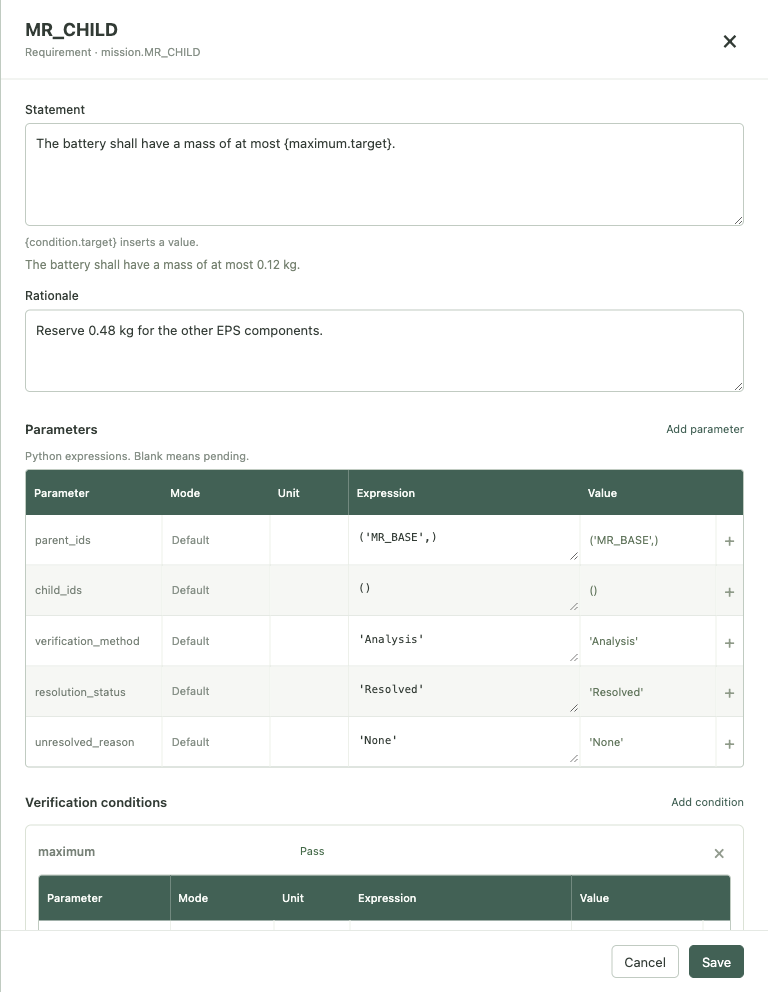
\includegraphics[width=0.90\linewidth,height=0.76\textheight,keepaspectratio]{fig/user-trials/mop01-club.png}
\caption[Enlarged requirement submission from MOP-01.]{Enlarged MOP-01 submission by the student club member, showing retained requirement fields and the verification condition status.}
\label{fig:user-trial-requirement-detail}
\end{figure}
\clearpage

\begin{figure}[p]
\centering
\footnotesize
\setlength{\tabcolsep}{0pt}
\begin{tabular}{@{}p{0.48\linewidth}@{\hspace{0.04\linewidth}}p{0.48\linewidth}@{}}
\textbf{Mission change} & \textbf{Requirement change} \\
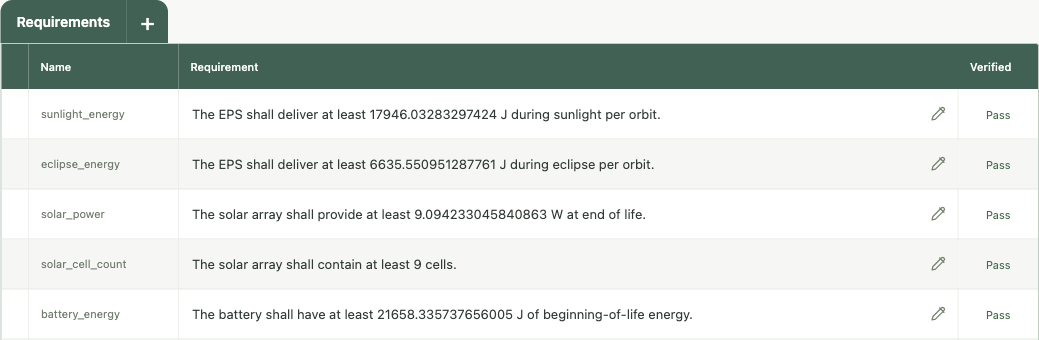
\includegraphics[width=\linewidth]{fig/user-trials/mop06-club-mission.png} & 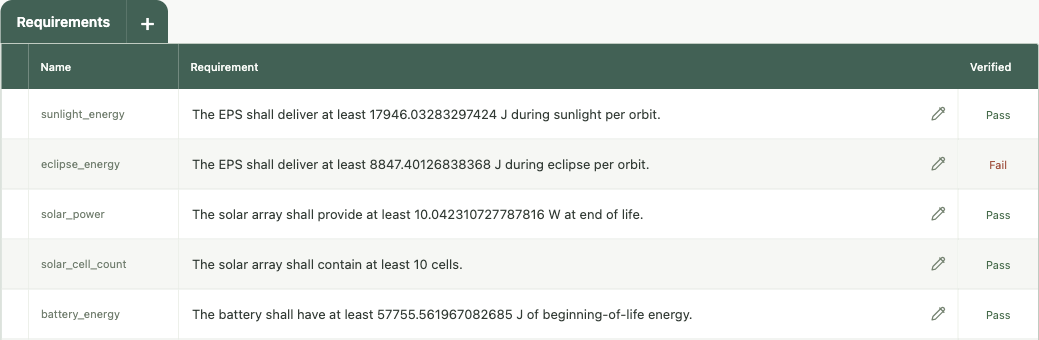
\includegraphics[width=\linewidth]{fig/user-trials/mop06-club-requirement.png} \\[6pt]
\textbf{Component change} & \textbf{Model change} \\
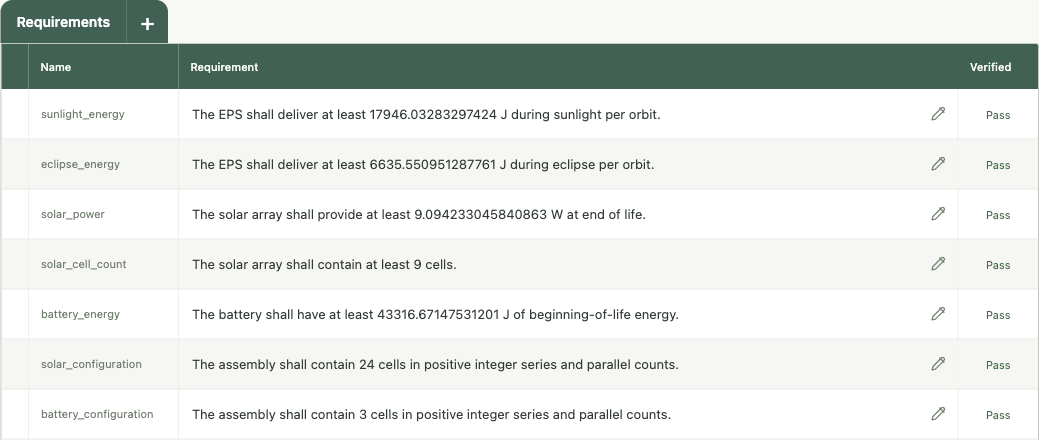
\includegraphics[width=\linewidth]{fig/user-trials/mop06-club-component.png} & 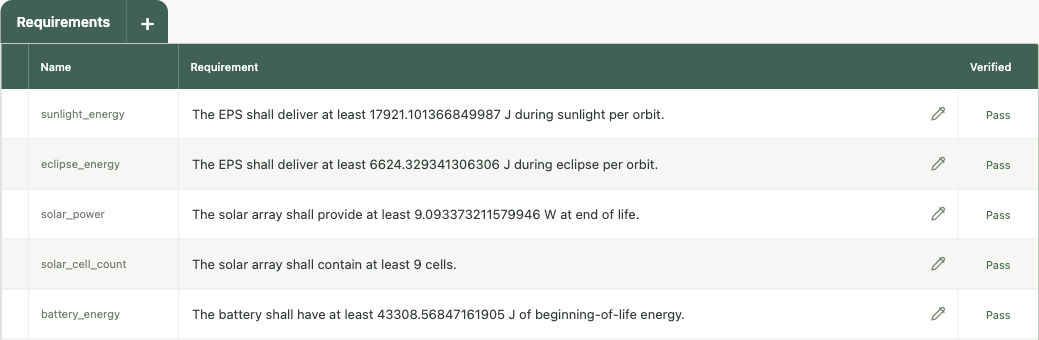
\includegraphics[width=\linewidth]{fig/user-trials/mop06-club-model.png} \\
\end{tabular}
\caption[MOP-06 intermediate change views.]{Student club member's intermediate screenshots for the four separate MOP-06 variations. Each preceding edit was restored before the next variation. The task clock continued through these captures and stopped at the final submission screenshot.}
\label{fig:user-trial-change-checkpoints}
\end{figure}
\clearpage

